%%%%
%% This Source Code Form is subject to the terms of the MIT License. 
%% If a copy of the MIT was not distributed with this file, You can obtain one at https://opensource.org/licenses/mit
%%
%% Last update: 2021/07/12
%% 
%% author: Dorian Gouzou <jackred@tuta.io>
%% repository hosted on github at https://github.com/jackred/Heriot_Watt_Thesis_Template
%%%%
\documentclass[12pt,a4paper]{report}

\usepackage{graphicx} % include graphics
\usepackage{fancyhdr} % layout
\usepackage[utf8]{inputenc}
\usepackage[T1]{fontenc} % font
\usepackage{setspace} % spacing
% \usepackage[left=4cm,right=2cm,top=2cm,bottom=2cm]{geometry}
\usepackage{mathptmx} % looks like times new roman
\usepackage{slantsc}
\usepackage{titlesec}
\usepackage{mfirstuc} 
\usepackage{calc}% http://ctan.org/pkg/calc
\usepackage{setspace}
\usepackage[acronym, nonumberlist]{glossaries} % https://www.overleaf.com/learn/latex/Glossaries
\usepackage[defernumbers=true]{biblatex}
\usepackage{hyperref} % https://ctan.org/pkg/hyperref
\usepackage{pdfpages}
\usepackage{float}

%% prefer than direct use in usepackage geometry
%% A4 layout in point is % 595x842

%% default value
\setlength{\hoffset}{0pt}
\setlength{\voffset}{0pt}

%% height
%% 72 - 60 + 20 + 25 = 57
\setlength{\topmargin}{-60pt}
\setlength{\headheight}{20pt}
\setlength{\headsep}{25pt}

\setlength{\footskip}{30pt}

%% width
%% 72 + 32 + 10 = 114pt = 40mm
\setlength{\oddsidemargin}{32pt}
\setlength{\evensidemargin}{32pt}
\setlength{\marginparsep}{10pt}

%% size text
\setlength{\textheight}{728pt}
\setlength{\textwidth}{425pt}

%% style
%% preliminary, just roman pagination + empty header
\fancypagestyle{preliminary}{
    \renewcommand{\headrulewidth}{0pt}
    \fancyhead[RCL]{}

    \pagenumbering{Roman}
}
%% chapter/classic text style
\fancypagestyle{chapter}{
    %% title of the chapter, left header, no uppercase, 10 pt, italics, no bold
    \fancyhead[L]{\normalfont\itshape\fontsize{10pt}{12pt}\selectfont\nouppercase{\leftmark}}
    \fancyhead[R]{}

    \fancyfoot[C]{\thepage}
    \renewcommand{\headrulewidth}{0.4pt}
    \renewcommand{\footrulewidth}{0pt}
    \pagenumbering{arabic}
}

%% define length and scaling for baseline
\newcommand{\headingBaseline}{12}
\newcommand{\headingBaselineDiv}{10}
\newlength{\chapterFontSize}
\newlength{\sectionFontSize}
\newlength{\subsectionFontSize}
\newlength{\chapterBaseline}
\newlength{\sectionBaseline}
\newlength{\subsectionBaseline}

%% change those value if you want to change the chapter/section/subsection font size
\setlength{\chapterFontSize}{14pt}
\setlength{\sectionFontSize}{12pt}
\setlength{\subsectionFontSize}{12pt}

%% automatic computation for baseline, rule of thumb is 1.2
\setlength{\chapterBaseline}{ \chapterFontSize * \headingBaseline / \headingBaselineDiv}
\setlength{\sectionBaseline}{ \sectionFontSize * \headingBaseline / \headingBaselineDiv}
\setlength{\subsectionBaseline}{ \subsectionFontSize * \headingBaseline / \headingBaselineDiv}


%% headings
%% Chapter, capitalised initial letter, 14-point, bold
\titleformat{\chapter}[display]
    {\normalfont\bfseries\fontsize{\chapterFontSize}{\chapterBaseline}\selectfont}{\chaptertitlename\ \thechapter}{14pt}{\capitalisewords}
%% left|above|below
\titlespacing{\chapter}{0pt}{10pt}{25pt}

%% Section, capitalised initial letter, 12-point
\titleformat{\section}[hang]
    {\normalfont\fontsize{\sectionFontSize}{\sectionBaseline}\selectfont}{\thesection}{5pt}{\capitalisewords}
%% left|above|below
\titlespacing{\section}{0pt}{25pt}{15pt}

%% Subsection, 12-point, italic
\titleformat{\subsection}[hang]
    {\normalfont\itshape\fontsize{\subsectionFontSize}{\subsectionBaseline}\selectfont\MakeLowercase}{\thesubsection}{5pt}{\makefirstuc}
%% left|above|below
\titlespacing{\subsection}{0pt}{20pt}{10pt}
  

%% table of content
\renewcommand{\contentsname}{Table of Contents}
\setcounter{tocdepth}{2} 

%% list of figure
\renewcommand*\listfigurename{Figure table}

%% init gloassaries
\makenoidxglossaries

%% bibliography config
%% https://tex.stackexchange.com/a/6977
\DeclareBibliographyCategory{cited}
\AtEveryCitekey{\addtocategory{cited}{\thefield{entrykey}}}
\addbibresource{Bibliography.bib}
\nocite{*}

%% hyperref setup
\usepackage{hyperref}
\hypersetup{
    colorlinks = true,
    linkcolor = black, % normal internal links
    citecolor = blue, % bibliographical links
    urlcolor = blue, % linked urls
    filecolor = black % url which open local files
}

%% The title of Thesis                
\newcommand{\thesisTitle}{How to make a thesis following the guideline with more text to have two lines}
%% Number of Volume, if more than one
%% not sure how it works out with latex tbh
\newcommand{\numberVolume}{2}
%% The number of this volume
\newcommand{\actualVolume}{1}
%% The author's name (you)
\newcommand{\authorName}{A Good Name}
%% Distinctions/Qualifications if desired
\newcommand{\distinction}{The awesome}   
%% The qualification  
\newcommand{\degreeQualification}{Doctor of Philosophy}
%% The institution
\newcommand{\institution}{Some weird institute no one ever heard about}
%% The school
\newcommand{\school}{School of Latex and Writing}
\newcommand{\university}{Heriot-Watt University}
%% Month of submission
\newcommand{\monthDate}{September}
%% Year of submission
\newcommand{\yearDate}{2042}

\newacronym{gcd}{GCD}{Greatest Common Divisor}
\newacronym{lcm}{LCM}{Least Common Multiple}
\usepackage{subfiles}
 % some package need to be loaded last in preamble

\begin{document}

\pagestyle{empty}
\begin{center}
\vspace*{15pt}\par

\begin{spacing}{1.8}
%% you can replace by \MakeUppercase if you want uppercase
{\Large\bfseries\MakeLowercase{\capitalisewords{\thesisTitle}}}
\end{spacing}

% This thesis is composed of \numberVolume volumes. This one is the number \actualVolume.

\vspace{50pt}\par

{\itshape\fontsize{15.5pt}{19pt}\selectfont by}\vspace{15pt}

{
\Large \authorName
% , \distinction
}

\vspace{50pt}\par

{
\fontsize{15pt}{18pt}\selectfont Submitted for the degree of \\ \vspace{8pt} \fontsize{16pt}{19pt}\selectfont\degree
}

\vspace{140pt}\par


{\scshape\large\setstretch{1.5} \institution\\ \school\\ \university\\
}

\vspace{80pt}\par


{\Large \monthDate\ \yearDate}

\vfill

\begin{flushleft}
\doublespacing
The copyright in this thesis is owned by the author. Any quotation from the thesis or use of any of the information contained in it must acknowledge this thesis as the source of the quotation or information.
\end{flushleft}
\end{center}

\clearpage
% % remove this line if you don't want pagination on preliminary pages
% % also read the comment below, for table of content and other
\pagestyle{preliminary}
\begin{center}
\LARGE\textbf {Abstract}
\end{center}
\vspace{5pt}

\noindent
In accordance with the Academic Regulations the thesis must contain an abstract preferably not exceeding 200 words, bound in to precede the thesis. The abstract should appear on its own, on a single page.  The format should be the same as that of the main text. The abstract should provide a synopsis of the thesis and shall state clearly the nature and scope of the research undertaken and of the contribution made to the knowledge of the subject treated. There should be a brief statement of the method of investigation where appropriate, an outline of the major divisions or principal arguments of the work and a summary of any conclusions reached. The abstract must follow the Title Page.
\clearpage
dedication
\clearpage
thanks everyone
\clearpage
% % read about declaration in file
% % Declaration statement

https://www.hw.ac.uk/students/studies/examinations/thesis.htm

This form should be placed after the Acknowledgements and bound into every copy of the thesis. Please note that the Student Service Centre will be unable to accept your thesis if the form is not bound into each submitted copy


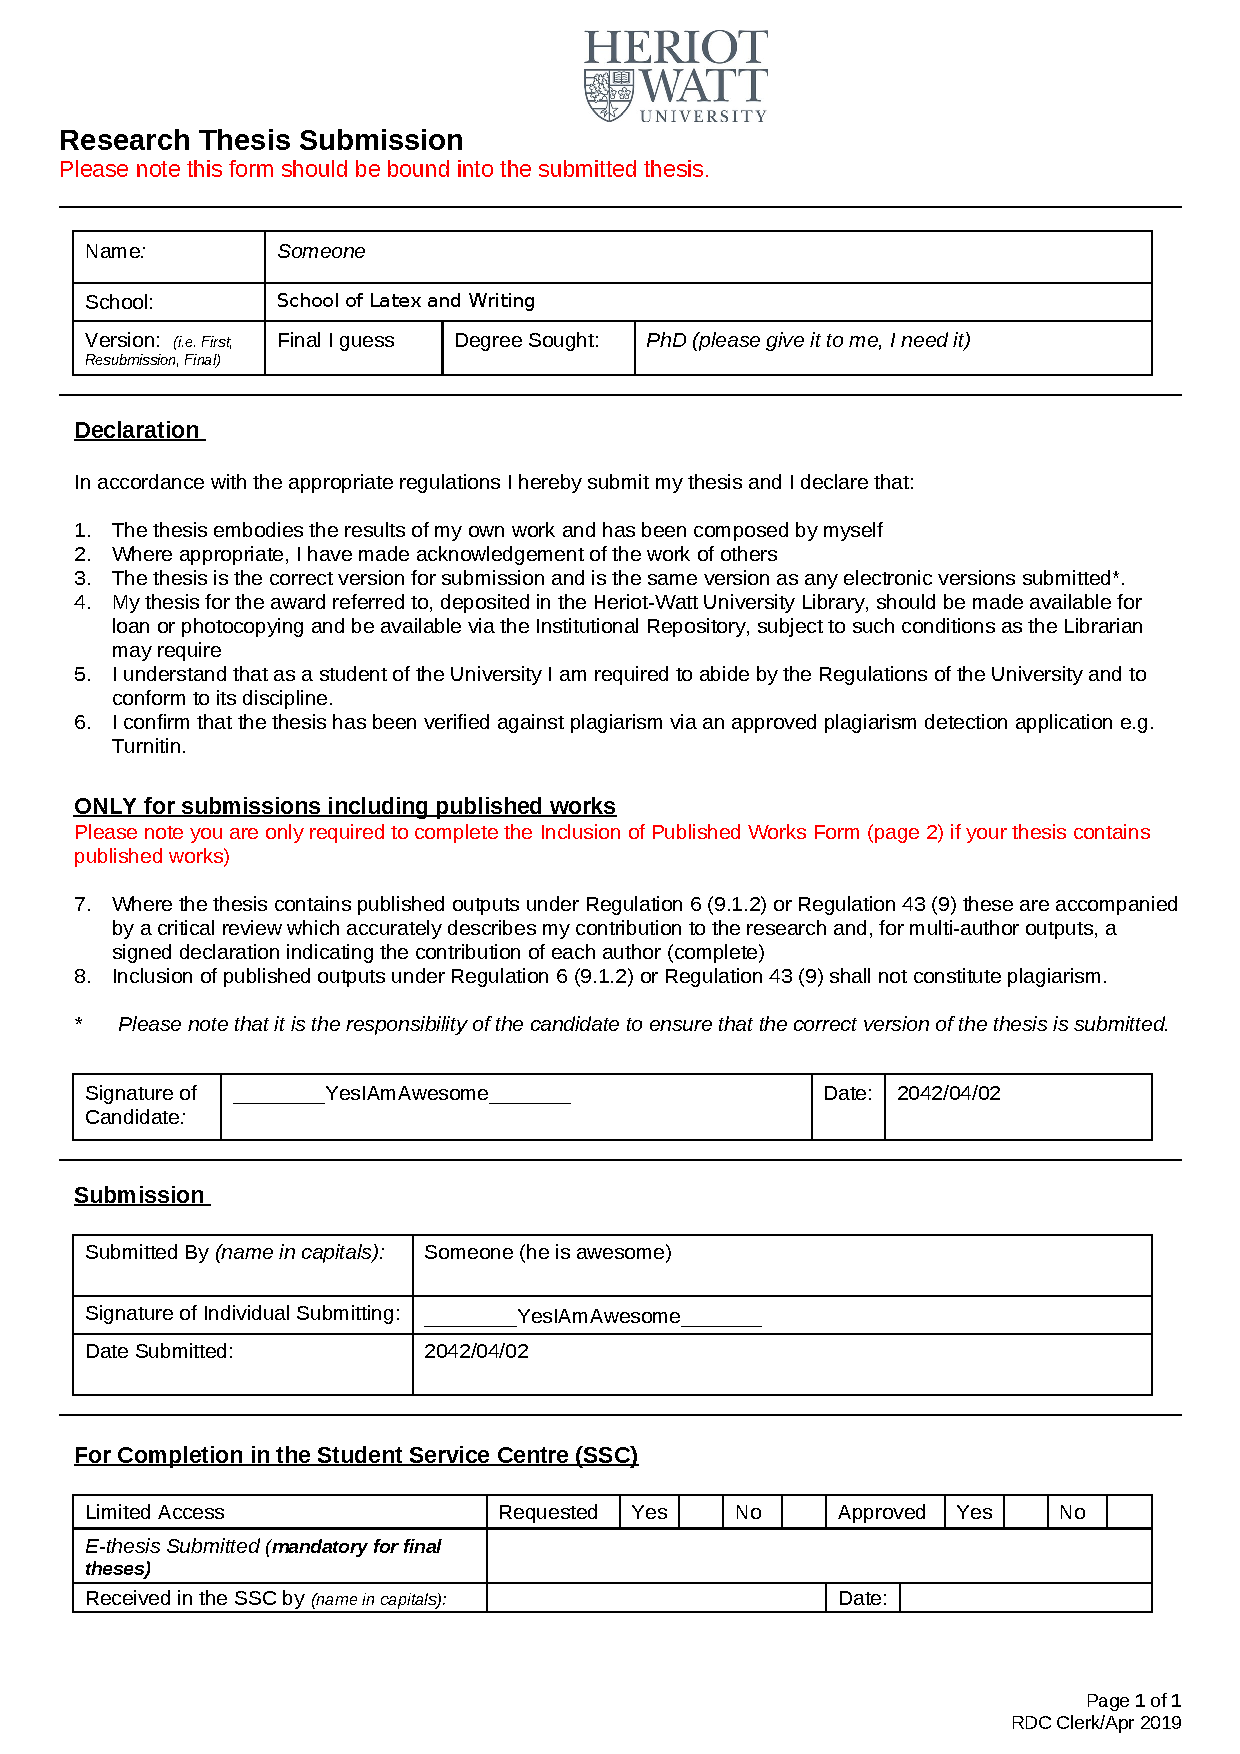
\includepdf[pages=-]{Preliminaries/5-declaration.pdf}

{
    \setstretch{1}
    \hypersetup{linkcolor=black}
    \tableofcontents
    \listoftables % optional
    \listoffigures % optional
    \glsaddall % this is to include all acronym. You can do a sort of citation for acronym and include only the one you use, Look at the glossary package for details.
    \printnoidxglossary[type=\acronymtype, title=Glossary] % optional
    %% put your publications in BibMine.bib 
    %% They will be displayed here
    \begin{refsection}[BibMine.bib]
    \DeclareFieldFormat{labelnumberwidth}{#1}
    \nocite{*}
    \printbibliography[omitnumbers=true,title={List of Publications}]
    \end{refsection}
}

%% if you don't want pagination you need to use this commented part instead of the one above for the table of content/list of figure/etc
%% this is because the toc is defined in an annoying way, especially multi page one
%% solution found here: https://tex.stackexchange.com/a/173423
% {
%     \hypersetup{linkcolor=black}
%     \pagestyle{empty}              % Removes numbers from middle pages.
%     \fancypagestyle{plain}         % Re-definition removes numbers from first page.
%     {
%         \fancyhf{}%                       % Clear all header and footer fields.
%         \renewcommand{\headrulewidth}{0pt}% Clear rules (remove these two lines if not desired).
%         \renewcommand{\footrulewidth}{0pt}%
%     }
%     \tableofcontents
%     \thispagestyle{empty}
%     \listoftables %optional
%     \thispagestyle{empty}
%     \listoffigures %optional
%     \thispagestyle{empty}
%     \glsaddall % this is to include all acronym. You can do a sort of citation for acronym and include only the one you use, Look at the glossary package for details.
%     \printnoidxglossary[type=\acronymtype, title=Glossary] % optional
%     \thispagestyle{empty}
%     %% put your publications in BibMine.bib 
%     %% They will be displayed here
%     \begin{refsection}[BibMine.bib]
%     \DeclareFieldFormat{labelnumberwidth}{#1}
%     \nocite{*}
%     \printbibliography[omitnumbers=true,title={List of Publications}]
%     \end{refsection}
%     \thispagestyle{empty}
% }



\clearpage

\pagestyle{chapter}
\subfile{Chapters/Chapter1-Introduction}
\subfile{Chapters/Chapter2}
\subfile{Chapters/Chapter3}
\appendix
\subfile{Appendices/Appendix1}

%% add publications in pdf format
\clearpage
\stepcounter{chapter}
\addcontentsline{toc}{chapter}{\thechapter\ \ \ \ Publication 1}
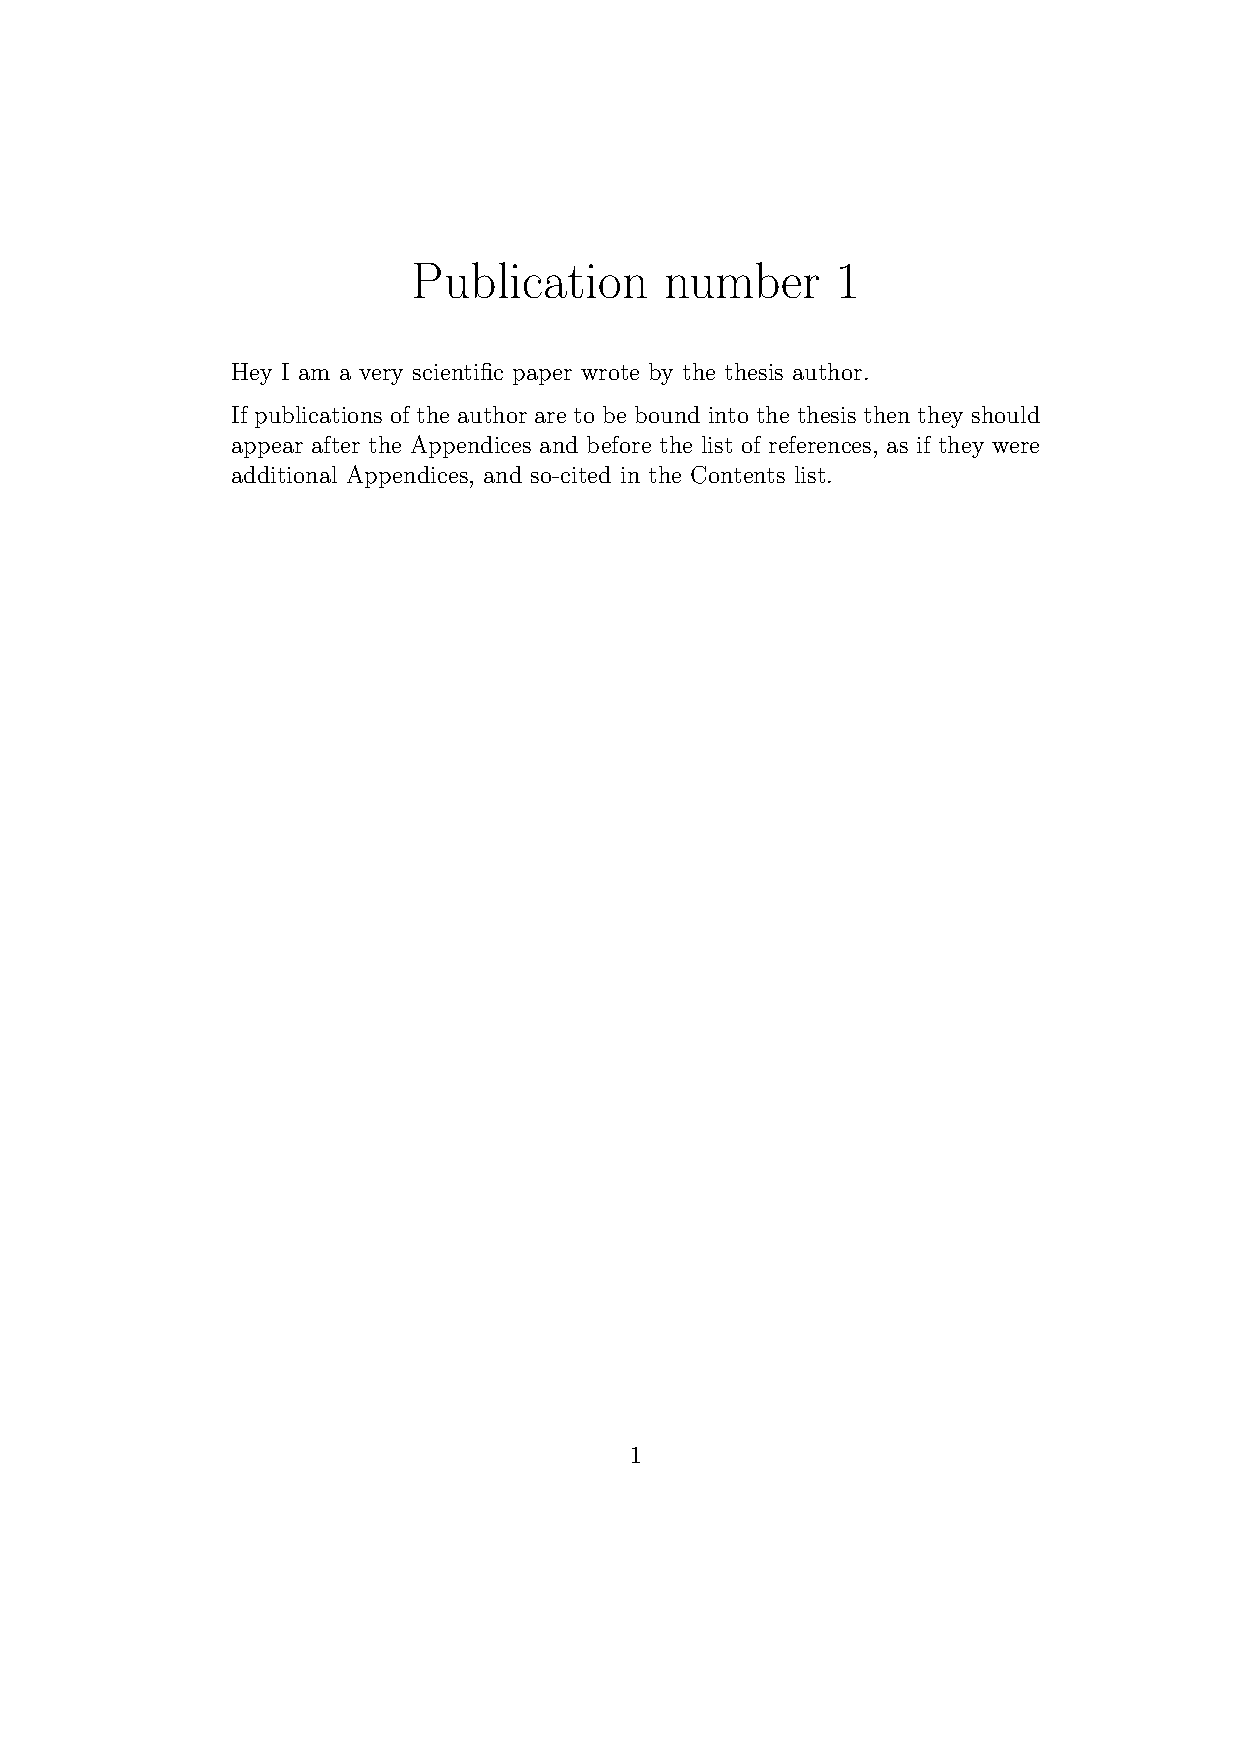
\includepdf[pages=-]{Publications/Publication1.pdf}


%% using biblatex rather than bibtex to easily have further reading and references
%% you need to remove the cache file when adding files to the bibliography
%% Log and output files > trash icons in Overleaf
%% sorted by citation
\label{Bibliography}
\printbibliography[title={References}, heading=bibintoc, resetnumbers=true]
%% sorted by alphabetical order, using author name
\begin{refsection}
\DeclareFieldFormat{labelnumberwidth}{#1}
\nocite{*}
\printbibliography[title={Bibliography}, notcategory=cited, omitnumbers=true, heading=bibintoc]
\end{refsection}

\end{document}
